\documentclass[11pt]{article}
\usepackage[scaled=0.92]{helvet}
\usepackage{geometry}
\geometry{letterpaper,tmargin=1in,bmargin=1in,lmargin=1in,rmargin=1in}
\usepackage[parfill]{parskip} % Activate to begin paragraphs with an empty line rather than an indent %\usepackage{graphicx}
\usepackage{amsmath,amssymb, mathrsfs, dsfont}
\usepackage{tabularx}
\usepackage[font=footnotesize,labelfont=bf]{caption}
\usepackage{graphicx}
\usepackage{xcolor}
%\usepackage[linkbordercolor ={1 1 1} ]{hyperref}
%\usepackage[sf]{titlesec}
\usepackage{natbib}
\usepackage{../../Tianpei_Report}


\begin{document}
\title{Self-study: Semi-discrete Optimal Transport}
\author{Tianpei Xie}
\date{ Aug. 19th., 2022 }
\maketitle
\tableofcontents
\newpage
\section{Optimal transport, entropy regularization, c-transform}
\begin{itemize}
\item For discrete measures, $\alpha = \sum_{i=1}^{n}a_i \delta_{\mb{x}_{i}}$ and $\beta := \sum_{i=1}^{m}b_i \delta_{\mb{y}_{i}}$, the primal problem for optimal transport is 
\begin{align}
\min_{\mb{P} \in \bR_{+}^{n \times m}} & \inn{\mb{P}}{\mb{C}} = \sum_{i,j}C_{i,j} P_{i,j} \label{eqn: optimal_transport_linear_prog}\\
\text{s.t. }&  \mb{P}\mb{1}_{m} = \mb{a} \label{eqn: optimal_transport_linear_constraint}\\
&\mb{P}^{T}\mb{1}_{n} = \mb{b}  \label{eqn: optimal_transport_linear_constraint2} \\
&P_{i,j} \ge 0 \nonumber
\end{align} where $\mb{C}_{n,m} := [C_{i,j}]_{i\in [1:n], j\in [1:m]}$,  $C_{i,j}:= c(\mb{x}_i, \mb{y}_j) \ge 0$. The feasible set is defined as
\begin{align}
U(\mb{a}, \mb{b}) := \set{\mb{P} \in \bR_{+}^{n \times m}: \mb{P}\mb{1}_{m} = \mb{a},\;\mb{P}^{T}\mb{1}_{n} = \mb{b}} \label{eqn: optimal_transport_feasible_set}
\end{align}

\item the corresponding dual problem with respect to primal problem is 
\begin{align}
\max_{\mb{\lambda} \in \bR^{n}, \mb{\mu} \in \bR^{m}} & \inn{\mb{\lambda}}{\mb{a}} + \inn{\mb{\mu}}{\mb{b}} \label{eqn: optimal_transport_dual}\\
\text{s.t. } & \lambda_i + \mu_{j} \le C_{i,j}\quad \forall\, i\in [1:n], j\in [1:m] \label{eqn: optimal_transport_dual_constraint}
\end{align} where $\mb{\lambda}= [\lambda_i]_{n}$, $\mb{\mu}= [\mu_{j}]_{m}$ are \textbf{dual variables} (slack variables) for marginal distribution constrain $\mb{a}$ and $\mb{b}$. We denote $\mb{\lambda}\oplus \mb{\mu}:= \mb{\lambda}\mb{1}_{m}^{T} + \mb{1}_{n}\mb{\mu}^{T} \in \bR^{n\times m}$ so that the linear constraints is $\mb{\lambda}\oplus \mb{\mu} \le \mb{C}$. Such dual variables $\mb{\lambda}$, $\mb{\mu}$ are often referred to as "\emph{\textbf{Kantorovich potentials}}."  The feasible set of the dual problem is defined as 
\begin{align}
R(\mb{C}) := \set{\mb{\lambda} \in \bR^{n}, \mb{\mu} \in \bR^{m}: \mb{\lambda}\oplus \mb{\mu} \le \mb{C}} \label{eqn: optimal_transport_dual_feasible_set}
\end{align} where $\mb{\lambda}\oplus \mb{\mu} = \mb{\lambda}\mb{1}_{m} + \mb{1}_n \mb{\mu}^{T}.$

\item The \textbf{probability interpretation} of orignal primal and dual Kantorovich optimal transport problem: 
\begin{align}
(P)\quad \cL_{c}(\alpha, \beta) = \min_{(X, Y) \sim \pi}& \E{(X,Y)}{c(X, Y)}   \label{eqn: optimal_transport_prob} \\
\text{s.t. }&  X \sim \alpha,  \nonumber \\
& Y\sim \beta  \nonumber
\end{align}
\begin{align}
(D)\quad \cL_{c}(\alpha, \beta) = \max_{(\lambda,  \mu) \in \in \cC(\cX)\times \cC(\cY)} & \E{X\sim \alpha}{\lambda(X)} + \E{Y \sim \beta}{\mu(Y)} \label{eqn: optimal_transport_dual_prob} \\
\text{s.t. }&  \lambda(x) + \mu(y) \le c(x, y),\quad \forall x\in \cX, y \in \cY, \nonumber
\end{align}

\item We also have the \textbf{entropic regularized optimal transport problem} 
\begin{align}
L_{\mb{C}}^{\epsilon}(\mb{a}, \mb{b}) = \min_{\mb{P} \in U(\mb{a}, \mb{b})} \inn{\mb{P}}{\mb{C}} - \epsilon H(\mb{P}) \label{eqn: optimal_transport_primal_entropy_reg}
\end{align} where the second term is entropy 
\begin{align}
H(\mb{P}) &:= -\sum_{i,j}P_{i,j}\paren{\log(P_{i,j}) - 1} \label{eqn: entropy_regularization}
\end{align} This problem has a unique optimal solution (maximum entropy optimal transport plan) 
\begin{align}
\mb{P}^{*} &= \diag{\mb{u}}\mb{K}\diag{\mb{v}}  \label{eqn: optimal_transport_primal_kl_sol2}
\end{align} where  $\mb{u} = [\exp(\lambda_i / \epsilon)] = \exp(\mb{\lambda}/\epsilon)$ and $\mb{v} =  [\exp(\mu_j / \epsilon)] = \exp(\mb{\mu}/\epsilon)$.

\item The dual problem of the \textbf{maximum entropy optimal transport problem}:
\begin{align}
L_{\mb{C}}^{\epsilon}(\mb{a}, \mb{b}) = \max_{\mb{\lambda} \in \bR^{n}, \mb{\mu} \in \bR^{m}}& \inn{\mb{\lambda}}{\mb{a}} + \inn{\mb{\mu}}{\mb{b}} - \epsilon \inn{\exp\paren{\mb{\lambda}/\epsilon}}{\mb{K}\exp\paren{\mb{\mu}/\epsilon}} \label{eqn: optimal_transport_dual_entropy_reg}
\end{align} where $\mb{K} = \exp\paren{-\mb{C}/\epsilon}$ is the Gibbs distribution. 



\item The \textbf{probability interpretation} of primal and dual maximum entropy optimal transport problem:
\begin{align}
(P)\quad \cL^{\epsilon}(\alpha, \beta) :=\min_{(X, Y) \sim \pi}& \E{(X,Y)}{c(X, Y)} + \epsilon\; I(X; Y) \label{eqn: optimal_transport_mutual_info} \\
\text{s.t. }& X\sim \alpha \nonumber\\
&Y \sim \beta \nonumber
\end{align} where $I(X; Y) :=  \kl{\pi}{\alpha\otimes \beta}$ is the mutual information between $X$ and $Y$.
\begin{align}
(D)\quad \cL^{\epsilon}(\alpha, \beta) := \sup_{(\lambda,\mu) \in \cC(\cX) \times \cC(\cY)} & \E{X \sim \alpha }{\lambda(X)}  + \E{Y \sim \beta}{\mu(Y)} \nonumber\\
& - \epsilon \E{X \sim \alpha, Y \sim \beta}{\exp\paren{\frac{-c(X,Y) + \lambda(X)+ \mu(Y)}{\epsilon}}}.  \label{eqn: optimal_transport_dual_entropy_prob}
\end{align}

\item Given a cost function $c: \cX \times \cY \rightarrow \bR_{+}$, $f: \cX \rightarrow \bR$, the \textbf{\emph{$c$-transform}} of $f$ is defined as
\begin{align}
f^{c}(y) &:= \inf_{x\in \cX}c(x, y) - f(x)  \label{eqn: c_transform}
\end{align} The function $f^{c}: \cY \rightarrow \bR$ is also called the \textbf{\emph{$c$-conjugate function}} of $f$. 
For discrete case, we have \textbf{\emph{$C$-transform vector}} for cost matrix $\mb{C} = [C_{i,j}]_{n \times m}$ and vector $\mb{f} = [f_1, \ldots, f_{n}] \in \bR^{n}$, 
\begin{align}
 \mb{f}_{j}^{\mb{C}} &:= \min_{i \in [1:n]}C_{i,j} - \mb{f}_{i} \label{eqn: c_transform_vector}
\end{align} The vector $\mb{f}^{\mb{C}} \in \bR^{m}$ is also called the \textbf{\emph{$C$-conjugate vector}} of $\mb{f}$.


Similarly, $g: \cY \rightarrow \bR$, the \textbf{\emph{$\bar{c}$-transform}} of $g$ is defined as
\begin{align}
g^{\bar{c}}(x) &:= \inf_{y\in \cY}c(x, y) - g(y)  \label{eqn: c_bar_transform}
\end{align} 
For discrete case, we have \textbf{\emph{$\bar{C}$-transform vector}} $\mb{g}^{\bar{\mb{C}}} \in \bR^{n}$ for cost matrix $\mb{C} = [C_{i,j}]_{n \times m}$ and vector $\mb{g} = [g_1, \ldots, g_{m}] \in \bR^{m}$, 
\begin{align}
 \mb{g}_{i}^{\bar{\mb{C}}} &:= \min_{j \in [1:m]}C_{i,j} - \mb{g}_{j} \label{eqn: c_bar_transform_vector}
\end{align}


A function $\psi: \cX \rightarrow \bR$ is \textbf{$c$-concave} if there exists some function $\phi: \cY \rightarrow \bR$ and cost function $c: \cX \times \cY \rightarrow \bR_{+}$ so that $\psi$ is the $\bar{c}$-transform of $\phi$, i.e. 
$\psi = \phi^{\bar{c}}$. Denote $\psi$ as $c$-concave($\cX$).

A function $\phi: \cY \rightarrow \bR$ is \textbf{$\bar{c}$-concave} if there exists some function $\psi: \cX \rightarrow \bR$ and cost function $c: \cX \times \cY \rightarrow \bR_{+}$ so that $\phi$ is the $c$-transform of $\psi$, i.e. 
$\phi = \psi^{c}$. Denote $\phi$ as $\bar{c}$-concave($\cY$)

For distance $c=d$, $f^{c} = f^{\bar{c}}$, thus we drop their distinctions.

\item Suppose that $c: \cX \times \cY \rightarrow \bR_{+}$ is real valued. 
\begin{enumerate}
\item For any $f_1: \cX \rightarrow \bR$ and $f_2: \cX \rightarrow \bR$, $f_{1} \le f_{2},\Leftrightarrow\;    f_{1}^{c} \ge f_{2}^{c}$
\item For any $f: \cX \rightarrow \bR$ and $g: \cY \rightarrow \bR$, $f^{c\bar{c}} \ge f, \;  g^{\bar{c}c} \ge g$ In general, $f^{c\bar{c}}$ is the \textbf{smallest $c$-concave function} larger than $f$
\item $f^{c\bar{c}c} =  f^{c}$ and $g^{\bar{c}c\bar{c}} =  g^{\bar{c}}$; in other words, $f^{c\bar{c}} = f$ if and only if $f$ is a $c$-concave function
\end{enumerate}


\item 
\begin{proposition}
If $c: \cX \times \cX\rightarrow \bR$ is a distance, then the function $f: \cX \rightarrow \bR$ is \textbf{$c$-concave} if and only if $f$ is \textbf{Lipschitz continuous} with Lipschitz constant less than $1$ w.r.t. the distance $c$.  We will denote by $\text{Lip}_1$ the set of these functions. Moreover, for every $f \in \text{Lip}_1$, i.e. $\norm{f}{L} \le 1$, we have the $c$-transform of $f$, $f^{c} = -f$. \citep{santambrogio2015optimal}
\end{proposition}

\item Thus the dual problem \eqref{eqn: optimal_transport_dual} is equivalent to an \textbf{unconstrained optimization problem}
\begin{align}
\cL_{c}(\alpha, \beta)&:= \max_{\lambda \in \cC(\cX)} \int_{\cX}\lambda d\alpha + \int_{\cY} \lambda^{c} d\beta   \label{eqn: optimal_transport_dual_c_transform_prob} \\
&= \max_{\mu \in  \cC(\cY)} \int_{\cX}\mu^{\bar{c}} d\alpha + \int_{\cY} \mu d\beta  \label{eqn: optimal_transport_dual_c_concave_prob}
\end{align}
\end{itemize}


\section{Semidiscrete optimal transport}
\begin{figure}
\begin{minipage}[t]{1\linewidth}
  \centering
  \centerline{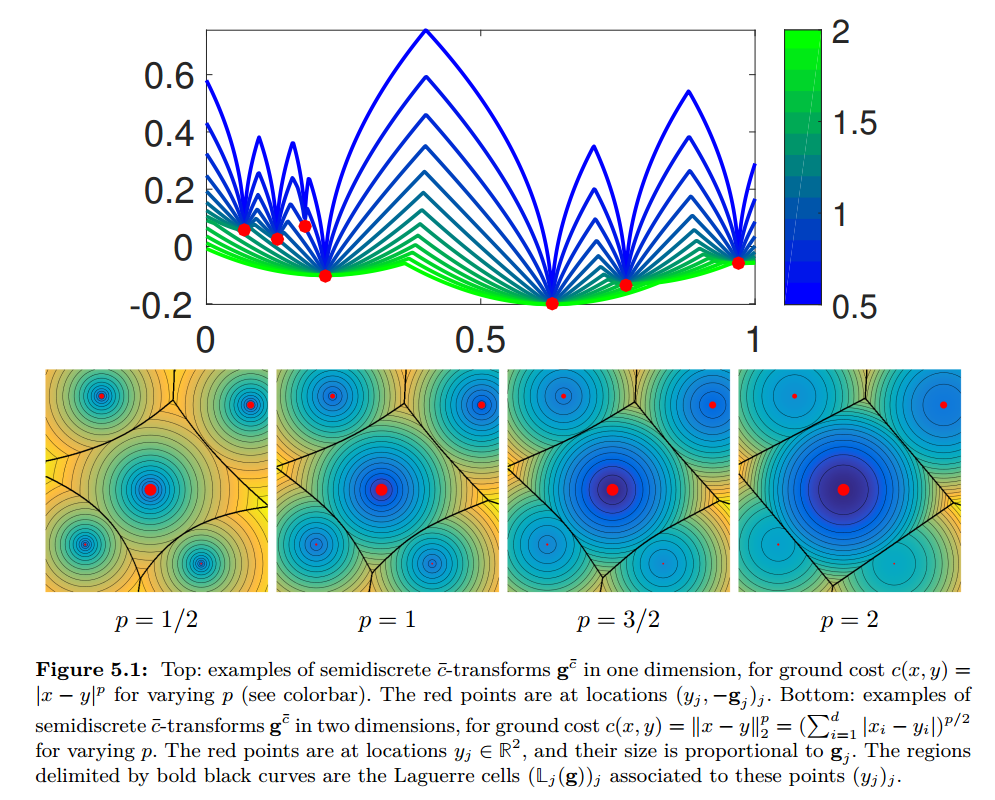
\includegraphics[scale = 0.35]{c_bar_transform_semidiscrete.png}}
    \vspace{-3pt}
  \centerline{(a)}
\end{minipage}\\[-5pt]
\begin{minipage}[t]{1\linewidth}
  \centering
  \centerline{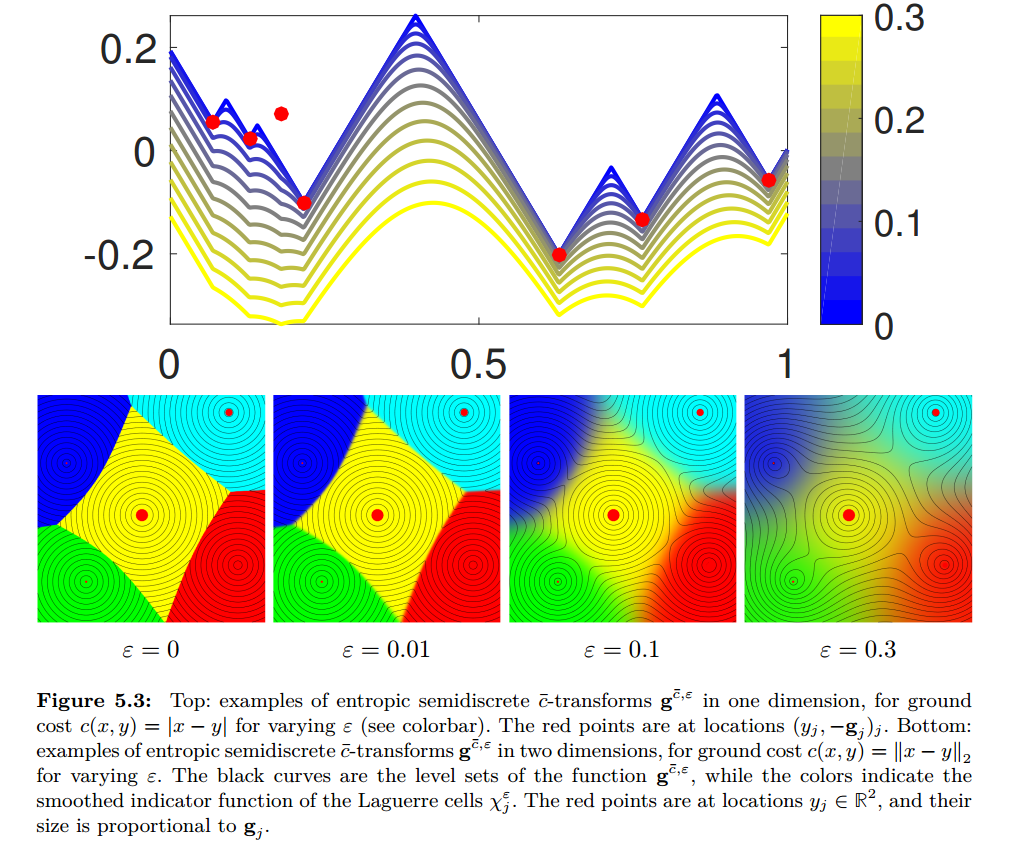
\includegraphics[scale = 0.32]{c_bar_transform_semidiscrete_ent.png}}\
  \vspace{-3pt}
   \centerline{(b)}
\end{minipage}
\caption{\footnotesize{\textbf{(a) The $\bar{c}$-transform of semidiscrete measures. (b)The $\bar{c}$-transform of semidiscrete measures with entropic regularization}}}
\label{fig: c_bar_transform_semidiscrete}
\end{figure}



\subsection{semidiscrete problem formulation}
Given discrete measure $\beta := \sum_{i=1}^{m}b_i \delta_{\mb{y}_{i}}$, the $\bar{c}$-transform of dual potential $\mb{\mu}$ is defined by restricting the minimization to the support $(\mb{y}_{i})$ of $\beta$
\begin{align}
\mb{\mu}^{\bar{c}}(\mb{x}) &= \min_{j=1,\ldots, m}\paren{c(\mb{x}, \mb{y}_j) - \mu_{j}}, \quad \forall \mb{x}\in \cX, \forall \mb{\mu} \in \bR^{m} \label{eqn: c_bar_transform_semidiscrete}
\end{align} Note that this is imposing that the support of $\beta$ is equal to $\cX$. The $\bar{c}$-transform map a vector $\mb{\mu}$ to $\mb{\mu}^{\bar{c}}(\mb{x})  \in \cC(\cX)$, a smooth function on $\cX$.

With $\bar{c}$-transform, we can apply the unconstrained dual formulation \eqref{eqn: optimal_transport_dual_c_concave_prob} and the problem becomes
\begin{align}
\cL_{c}(\alpha, \beta)&:=  \max_{\mu \in  \cC(\cY)} \int_{\cX}\mu^{\bar{c}} d\alpha + \int_{\cY} \mu d\beta \nonumber\\
&= \max_{\mb{\mu}  \in  \bR^{m}} \int_{\cX}\mb{\mu}^{\bar{c}}(\mb{x}) d\alpha(\mb{x}) + \inn{\mb{\mu}}{\mb{b}} \label{eqn: semidiscrete_optimal_transport}
\end{align}

We can define the \textbf{Laguerre cells} associated to the dual weights $\mb{\mu}$
\begin{align}
\bL_{j}(\mb{\mu}) &:= \set{\mb{x} \in \cX: c(\mb{x}, \mb{y}_{j}) - \mu_{j} \le c(\mb{x}, \mb{y}_{j'}) - \mu_{j'}, \;\;   \forall j' \neq j} \label{eqn: laguerre_cell_dual_c_bar}\\
& = \set{\mb{x} \in \cX: \mb{\mu}^{\bar{c}}(\mb{x}) = c(\mb{x}, \mb{y}_j) - \mu_{j}} \nonumber
\end{align} We see that $\cX = \bigcup_{j=1}^{m}\bL_{j}$, also $\bL_{j} \cap \bL_{j'} = \emptyset$. Therefore $\set{\bL_{j}, j=1,\ldots,m}$ is a \underline{\textbf{partition}} of $\cX$. When $\mb{\mu}$ is constant, the Laguerre cells decomposition corresponds to the \textbf{\emph{Voronoi diagram}} \emph{partition} of the space. Each cell corresponds to a discrete mass $(b_j, \mb{y}_j)$ of $\beta$.

This allows one to conveniently rewrite the minimized energy in \eqref{eqn: semidiscrete_optimal_transport} as
\begin{align}
\cE(\mb{\mu})&:=  \sum_{j=1}^{m}\int_{\bL_{j}(\mb{\mu}) }\paren{c(\mb{x}, \mb{y}_j) - \mu_{j}} d\alpha(\mb{x}) + \inn{\mb{\mu}}{\mb{b}}  \label{eqn: semidiscrete_optimal_transport_partition_obj}
\end{align}

The gradient of this objective function is 
\begin{align}
\grad{\mb{\mu}}{\cE(\mb{\mu})} &= \brac{-\int_{\bL_{j}(\mb{\mu}) }d\alpha(\mb{x})  + b_{j}}_{j=1}^{m}  \label{eqn: semidiscrete_grad}
\end{align} We can see that the gradient of objective w.r.t. dual potential $\mb{\mu}$ is the \textbf{difference} between the \textbf{discrete measure} $b_j$ at location $\mb{y}_j$ and the probabilty \textbf{measure of Laguerre} $\bL_{j}(\mb{\mu})$ associated with $(b_j, \mb{y}_j)$ (i.e. \textbf{hard assignment}). Figure \ref{fig: c_bar_transform_semidiscrete} shows the Laguerre cell partition of the space. Given this simple form of gradient, we can directly compute the solution using gradient descent. Figure \ref{fig: semidiscrete_ot_iteration} shows the iterations of gradient desent algorithm and its change of Laguerre cells.

\begin{figure}
\begin{minipage}[t]{1\linewidth}
  \centering
  \centerline{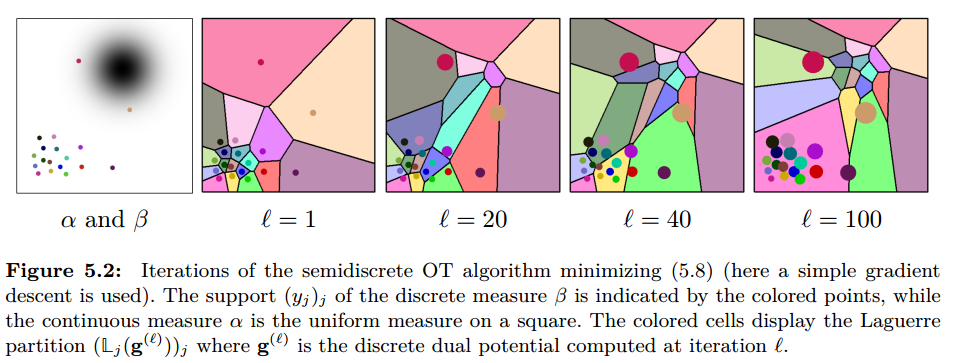
\includegraphics[scale = 0.4]{semidiscrete_ot_iteration.png}}
\end{minipage}
\caption{\footnotesize{\textbf{The iteration of gradient descent algorithm and the change of Laguerre cells \citep{gabriel2019computational}}}}
\label{fig: semidiscrete_ot_iteration}
\end{figure}
In the special case $c(x, y) = \norm{x - y}{2}^2$, the decomposition in Laguerre cells is also known as a \textbf{\emph{power diagram}}, which is a concept in \emph{\textbf{computational geometry}}. The cells are polyhedral and can be computed efficiently using computational geometry algorithms; see \citep{aurenhammer1987power}. The most widely used algorithm relies on the fact that the power diagram of points in $\bR^d$ is equal to the
projection on $\bR^d$ of the convex hull of the set of points $(\mb{y}_j, \norm{\mb{y}_j}{2}^2 - g_j)_{j=1}^{m} \subset R^{d+1}$. The semidiscrete
OT solver can be used in computational geometry. It is also used for solving the Monge-Amp\`ere equation. 

\subsection{K-means via semi-discrete optimal transport}
The k-means algorithm can be re-formulated using the semi-discrete optimal transport. In particular, $\beta = \sum_{i=1}^{k}a_i \delta_{\mb{c}_i}$ is constrained to be a \textbf{discrete measure} with a finite support of \textbf{size up to} $k$. $\beta$ is continous on domain $\cX= \bR^{d}$, $c(x, y) = \norm{x - y}{2}^2$, we can find $\beta$ via solving the minimum Kantorvich distance estimation 
\begin{align*}
\min_{\beta \in \cM_{k, 1}(\cX)}& \cL_{c}(\beta, \alpha) = \cL_{c}( \alpha, \beta)
\end{align*} Indeed, one can easily show that the \textbf{\emph{centroids}} output $\{\mb{c}_{i}, i=1,\ldots, k\}$ by the k-means problem correspond to the \textbf{support} of the solution $\alpha$ and that its \emph{\textbf{weights}} $a_i$ correspond to the \textbf{fraction} of points in $\beta$ \emph{assigned to each centroid} \citep{canas2012learning}.

One can show that approximating $\cL \approx \cL^{\epsilon}$ using entropic regularization results in smoothed out assignments that appear in \textbf{soft-clustering} variants of k-means, such as \emph{mixtures of Gaussians}.

\subsection{Entropic regularization}
Recall from \eqref{eqn: optimal_transport_dual_entropy_prob} that the dual of entropic regularized optimal transport
\begin{align}
\cL^{\epsilon}(\alpha, \beta):= \max_{(\lambda,\mu) \in \cC(\cX) \times \cC(\cY)}\;& \int_{\cX}\lambda d\alpha + \int_{\cY}\mu d\beta - \epsilon \int_{\cX \times \cY}\exp\paren{\frac{-c + \lambda\oplus \mu}{\epsilon}}d\alpha d\beta \label{eqn: optimal_transport_dual_entropy}
\end{align} Similarly to the unregularized problem \eqref{eqn: optimal_transport_dual_prob}, one can minimize explicitly with respect to either 
$\lambda$ or $\mu$ in \eqref{eqn: optimal_transport_dual_entropy}, which yields a\textbf{ \emph{smoothed} $c$-transform}
\begin{align}
\lambda^{c, \epsilon}(y) &= -\epsilon \log \int_{\cX}\exp\paren{\frac{-c(x, y) + \lambda(x)}{\epsilon}}d\alpha(x), \quad \forall  y \in \cY \label{eqn: smooth_c_transform}\\
\mu^{\bar{c}, \epsilon}(y) &= -\epsilon \log \int_{\cY}\exp\paren{\frac{-c(x, y) + \mu(y)}{\epsilon}}d\beta(y), \quad \forall  x \in \cX \label{eqn: smooth_c_bar_transform}
\end{align} Compare \eqref{eqn: c_transform} and \eqref{eqn: c_bar_transform} with \eqref{eqn: smooth_c_transform} and \eqref{fig: c_bar_transform_semidiscrete}, we see that instead of using $\min$ operation, in smooth $c$-transform, we use the \underline{$\text{soft-min}^{\epsilon}$} operator $\text{soft-min}^{\epsilon}(\mb{z}; \mb{b}) = - \epsilon\log \sum_i b_i \exp(-z_i/\epsilon)$ to maintain smoothness of the function. 

In the case of a discrete measure $\beta := \sum_{i=1}^{m}b_i \delta_{\mb{y}_{i}}$, the problem simplifies as with \eqref{eqn: c_bar_transform_semidiscrete} to a finite-dimensional problem expressed as a function of the discrete dual potential $\mb{\mu}$:
\begin{align}
\mb{\mu}^{\bar{c},\epsilon}(\mb{x}) &= \text{soft-min}^{\epsilon}_{j=1,\ldots, m}\paren{c(\mb{x}, \mb{y}_j) - \mu_{j}; \mb{b}}, \quad \forall \mb{x}\in \cX, \forall \mb{\mu} \in \bR^{m} \label{eqn: smooth_c_bar_transform_semidiscrete} \\
&=  -\epsilon \log \sum_{j=1}^{m} b_{j} \exp\paren{\frac{-(c(\mb{x},  \mb{y}_{j}) - \mu_{j})}{\epsilon}}\nonumber
\end{align}

Similar to \eqref{eqn: semidiscrete_optimal_transport}, we can solve the uncontrained dual problem using the smooth $\bar{c}$-transfrom
\begin{align}
\cL_{c}^{\epsilon}(\alpha, \beta) &= \max_{\mb{\mu}  \in  \bR^{m}} \int_{\cX}\mb{\mu}^{\bar{c},\epsilon}(\mb{x}) d\alpha(\mb{x}) + \inn{\mb{\mu}}{\mb{b}} \label{eqn: semidiscrete_optimal_transport_ent}
\end{align}
The minimized energy is 
\begin{align}
\cE^{\epsilon}(\mb{\mu})&:= \set{\int_{\cX}\mb{\mu}^{\bar{c},\epsilon}(\mb{x})  d\alpha(\mb{x})+ \inn{\mb{\mu}}{\mb{b}}}  \label{eqn: semidiscrete_optimal_transport_ent_obj} \\
&=-\E{\alpha}{\epsilon \log \sum_{j=1}^{m} b_{j} \exp\paren{\frac{-(c(X,  \mb{y}_{j}) - \mu_{j})}{\epsilon}} } + \inn{\mb{\mu}}{\mb{b}}  \nonumber
\end{align} This is actually the \emph{expectation} of negative loss function of  \textbf{multiclass logistic regression problem} w.r.t. $\alpha$.  Note that the LR need to minimize the loss and this is to maximize the energy.   Therefore,  the dual representation of \emph{\textbf{semidiscrete optimal transport}} with \textbf{entropic regularization} is \emph{\textbf{equivalent}} to \textbf{multi-class logistic regression}. 

The gradient of this functional reads
\begin{align}
\grad{\mb{\mu}}{\cE^{\epsilon}(\mb{\mu})} &= \brac{-\int_{\cX}\sigma_{j}^{\epsilon}(\mb{x})d\alpha(\mb{x})  + b_{j}}_{j=1}^{m}  \label{eqn: semidiscrete_ent_grad} \\
\text{where }& \sigma_{j}^{\epsilon}(\mb{x}) = \frac{ \exp\paren{\frac{-(c(\mb{x},  \mb{y}_{j}) - \mu_{j})}{\epsilon}}}{\sum_{j} \exp\paren{\frac{-(c(\mb{x},  \mb{y}_{j}) - \mu_{j})}{\epsilon}}}\text{ is soft-min function}
\end{align} Note that compare to \eqref{eqn: semidiscrete_grad}, there is no hard partition of space $\cX$ into Laguerre cells since the smoothed potential function is supported on entire domain. Instead, we assign a point $\mb{x}$ to one region with probability $[\sigma_{j}^{\epsilon}(\mb{x}), j=1,\ldots, m] \in \Delta_{m}$, i.e. \textbf{soft-assignment}. The gradient is the \textbf{difference} between the \textbf{discrete measure} $b_j$ at location $\mb{y}_j$ and $\E{\alpha}{\sigma_{j}^{\epsilon}(X)}$, the expectation of assignment under $\alpha$. 

As stated above, the optimization of discrete $\beta$ w.r.t. continous $\alpha = \cN(m, \sigma^2)$ will result in models such as Gaussian mixtures. 

One of important property is that $\grad{\mb{\mu}}{\cE^{\epsilon}(\mb{\mu})}$ is $1/\epsilon$ Lipschitz, and the Hessian $H(\cE^{\epsilon}(\mb{\mu}))$  is finite and bounded. Similar to logistic regression, $\cE^{\epsilon}$ have the properties based on \textbf{\emph{self-concordance}}. We can solve the problem \eqref{eqn: semidiscrete_optimal_transport_ent} via \textbf{second-order methods} such as \emph{Newton's method}, \emph{quasi-Newton} such as \emph{L-BFGS}. 

Since both energy functions in  \eqref{eqn: semidiscrete_optimal_transport} and \eqref{eqn: semidiscrete_optimal_transport_ent} are the \emph{\textbf{expectation}} over $\alpha$, we can use \emph{stochastic gradient descent} algorithm to solve them.


\begin{figure}
\begin{minipage}[t]{1\linewidth}
  \centering
  \centerline{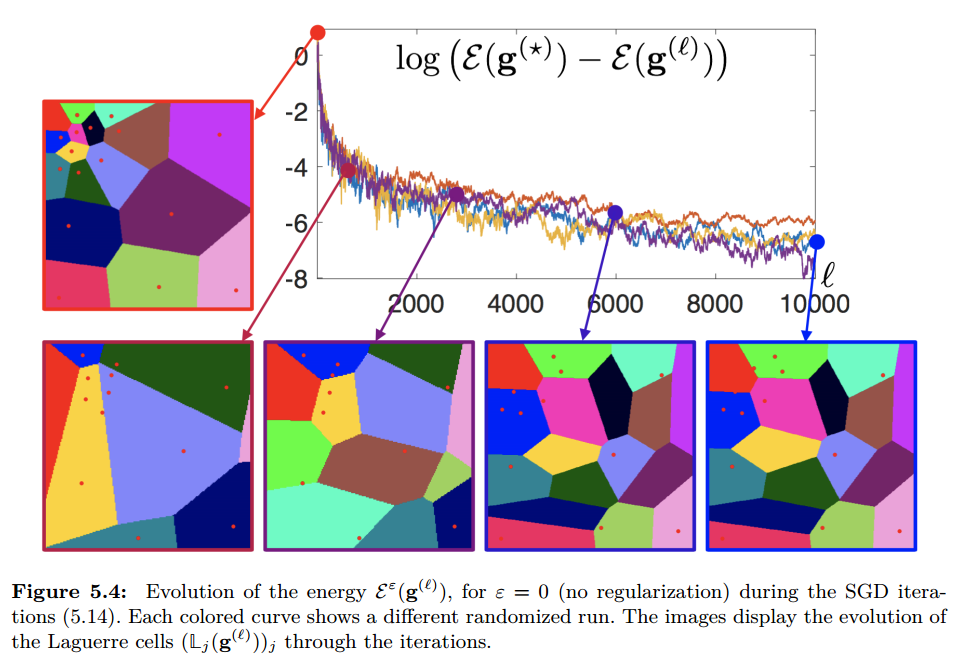
\includegraphics[scale = 0.4]{sgd_semidiscrete.png}}
\end{minipage}
\caption{\footnotesize{\textbf{The iteration of stochastic gradient descent algorithm and the change of Laguerre cells \citep{gabriel2019computational}}}}
\label{fig: sgd_semidiscrete}
\end{figure}

\newpage
\bibliographystyle{plainnat}
\bibliography{book_reference.bib}
\end{document}